\documentclass[
version=last,toc=bib,toc=graduated,toc=index,toc=listof,9pt,openany]{scrbook}
%\pdfminorversion=4
\usepackage[utf8]{inputenc}
\usepackage[english]{babel}
\usepackage{dejavu}

\usepackage{ifmtarg}
\usepackage{ifthen}
\usepackage{etoolbox} % \ifstrempty

\usepackage{geometry}
\geometry{%a6paper
paperwidth=125mm, paperheight=168mm, 
portrait,
top=22mm, inner=22mm, outer=20mm, bottom=25mm,
headsep=3mm, footskip=12mm
}

\usepackage{ragged2e} % nicer typesetting (hyphenation) for non raggedright and raggedleft
\usepackage{lscape}
\setlength{\parskip}{0pt}

\usepackage{relsize}

\clubpenalty=10000
\widowpenalty=10000 
\displaywidowpenalty=10000

\usepackage[letterspace=16]{microtype}

\usepackage{graphicx} % graphics

% search path for images
\graphicspath{{images-print/}{icons/}{extra-pages/}{wallpaper/}}
\usepackage{wrapfig}  % sponsor logos wrapped with text

\usepackage{tabu}
\usepackage{tabularx}
\usepackage{longtable}
\usepackage[table,cymk]{xcolor}
\usepackage{colortbl}

% embed PDF pages
% pdfpages must not be loaded before colortbl!
\usepackage{pdfpages}

\usepackage{multirow}
\usepackage{booktabs}
\usepackage{array}

\usepackage{refcount} % calculation of the page where the map is located

% page background
\usepackage[manualmark]{scrlayer-scrpage}
\pagestyle{scrplain}

\newcommand{\acro}[1]{{\textsmaller{#1}}} % macro for abbreviations with more than one capitalised letter

% headings in DejaVu Sans Condensed
\addtokomafont{sectioning}{\fontfamily{DejaVuSansCondensed-TLF}\selectfont}
\addtokomafont{pageheadfoot}{\usefont{T1}{DejaVuSansCondensed-TLF}{m}{n}}
\addtokomafont{pagenumber}{\usefont{T1}{DejaVuSansCondensed-TLF}{m}{n}}


% title/metadata
\title{State of the Map 2018}
\subtitle{Programme}
\author{OpenStreetMap Foundation}
\date{\today}

\clearscrheadings

% page numbers
\cfoot[\begin{small}\pagemark\end{small}]{\begin{small}\pagemark\end{small}}
\ofoot[]{}
\ifoot[]{}
\pagestyle{scrplain}

\linespread{1.15}

% include our custom macros
% command for a new time slot
\newcommand{\talktime}{9:99}
\newcommand{\newtimeslot}[1]{\newpage\renewcommand{\talktime}{#1}}

% new time slot but without a pagebreak
\newcommand{\newsmalltimeslot}[1]{\renewcommand{\talktime}{#1}}

% initialise \conferenceDay 
\newcommand{\conferenceDay}{Noday}


% define default page style (cutting marks with page number)
\DeclareNewLayer[background, oddorevenpage, width=125mm,%
height=169mm, contents={%
  
\includegraphics{wallpaper/crop-marks.pdf}%
}]{cropmarksevery}
\newpairofpagestyles[scrheadings]{cropmarksstyle}{}
\AddLayersAtBeginOfPageStyle{cropmarksstyle}{cropmarksevery}

% page style for title pages
\DeclareNewLayer[background, oddorevenpage, width=125mm,%
height=169mm, contents={%
  
\includegraphics{wallpaper/front-cover-with-crop-marks.pdf}%
}]{titlelayer}
\newpairofpagestyles[]{titlestyle}{}
\AddLayersAtBeginOfPageStyle{titlestyle}{titlelayer}

% define alias commands for all three days
\def\saturday{Saturday}
\def\sunday{Sunday}
\def\monday{Monday}

% define Saturday page style
\DeclareNewLayer[background, oddpage,  width=125mm,%
height=169mm, contents={%
  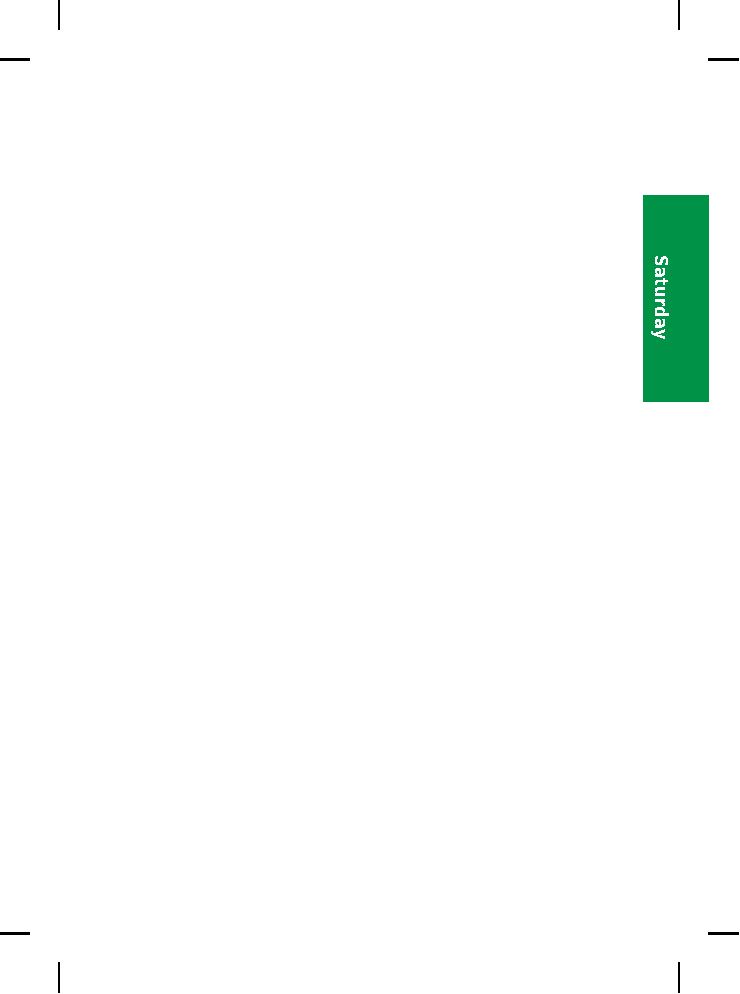
\includegraphics{wallpaper/saturday-odd.pdf}%
}]{saturdayodd}
\DeclareNewLayer[background, evenpage,  width=125mm,%
height=169mm, contents={%
  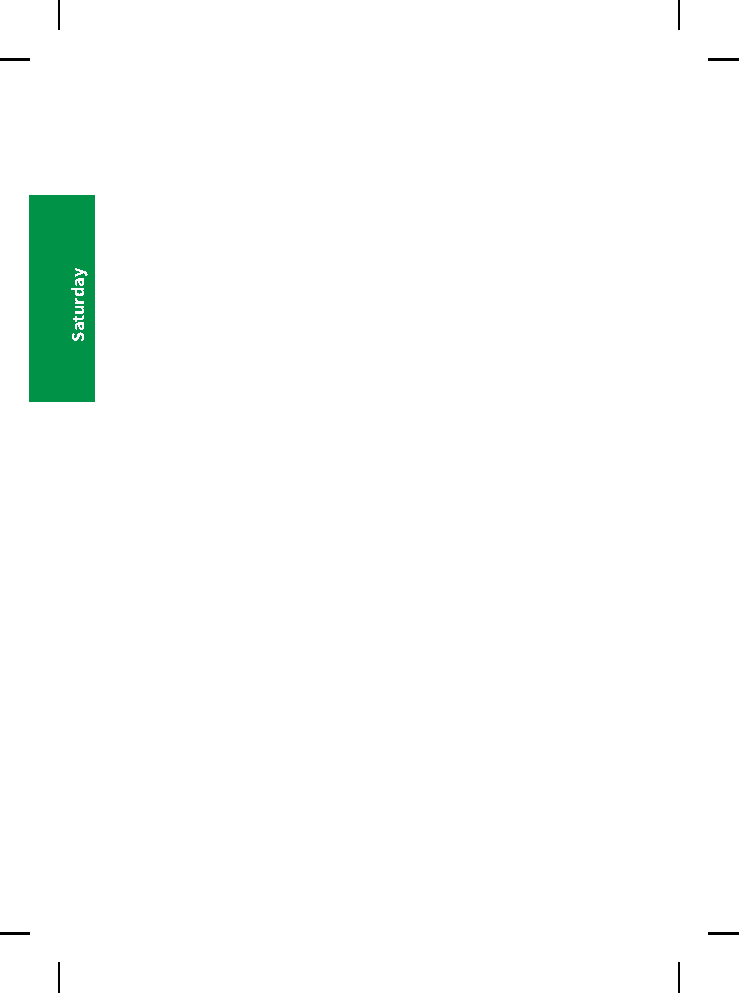
\includegraphics{wallpaper/saturday-even.pdf}%
}]{saturdayeven}
\DeclareNewLayer[background, oddpage,  width=125mm,%
height=169mm, contents={%
  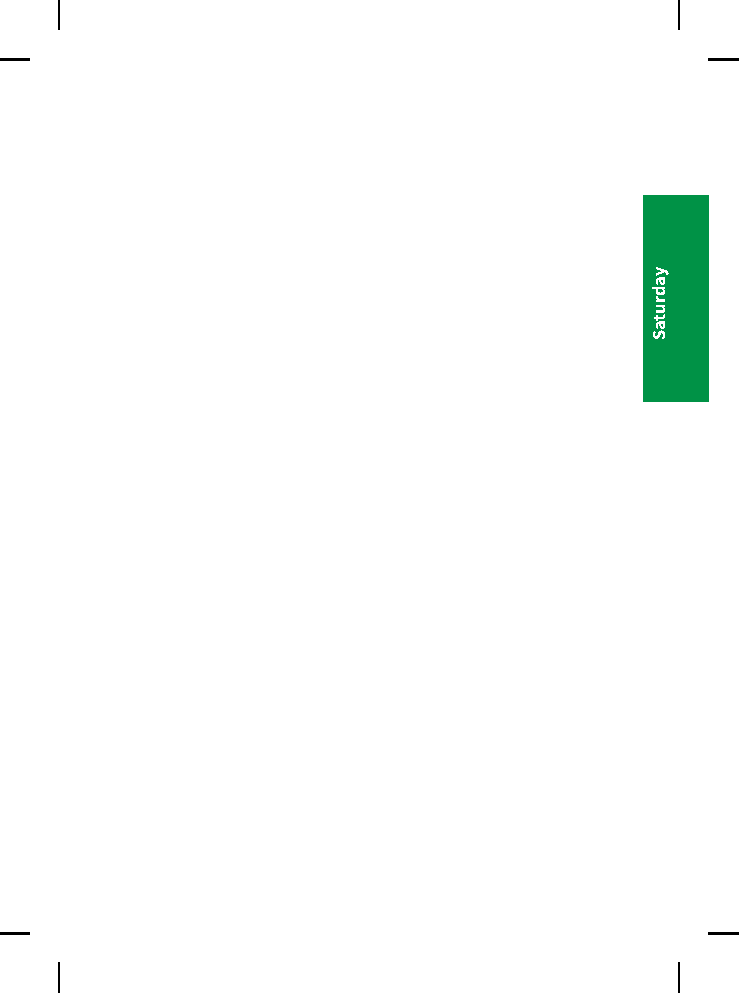
\includegraphics{wallpaper/saturday-odd-rotated.pdf}%
}]{saturdayoddrotated}
\newpairofpagestyles[scrheadings]{saturday-table}{}
\AddLayersAtBeginOfPageStyle{saturday-table}{saturdayeven}
\AddLayersAtBeginOfPageStyle{saturday-table}{saturdayoddrotated}
\newpairofpagestyles[scrheadings]{saturday}{}
\AddLayersAtBeginOfPageStyle{saturday}{saturdayeven}
\AddLayersAtBeginOfPageStyle{saturday}{saturdayodd}

% define Sunday page style
\DeclareNewLayer[background, oddpage,  width=125mm,%
height=169mm, contents={%
  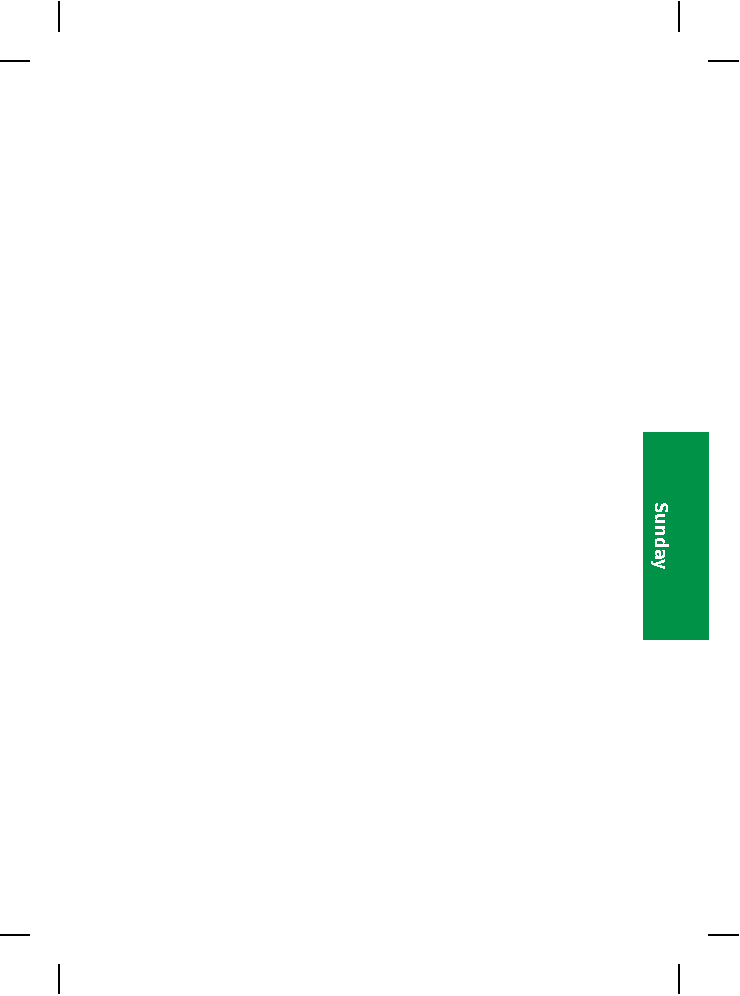
\includegraphics{wallpaper/sunday-odd.pdf}%
}]{sundayodd}
\DeclareNewLayer[background, evenpage,  width=125mm,%
height=169mm, contents={%
  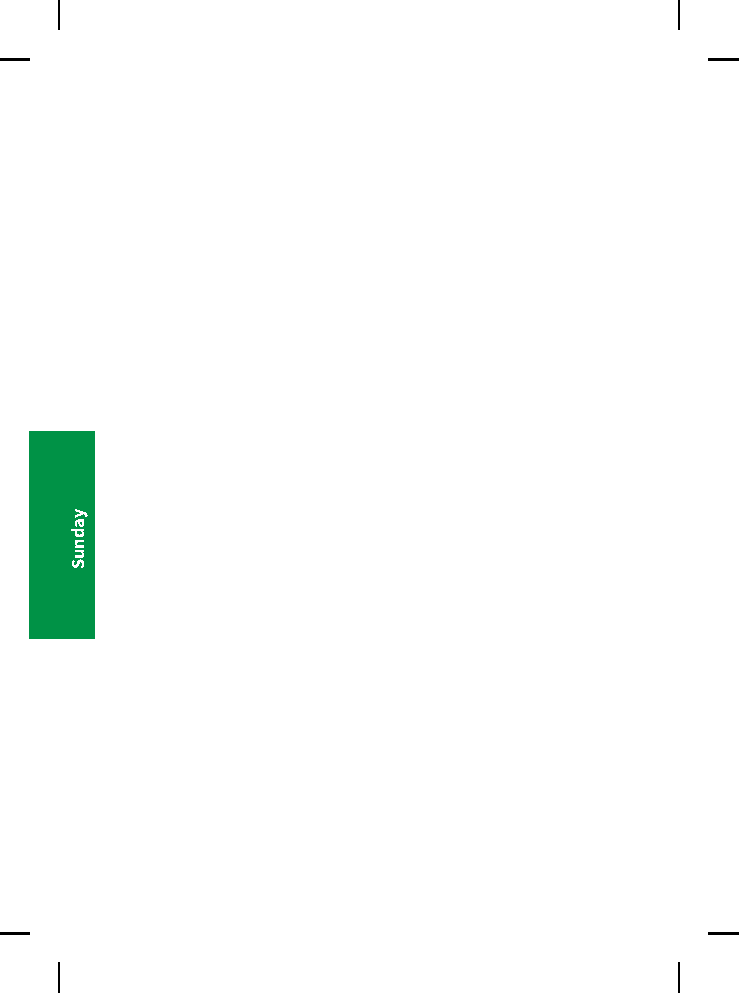
\includegraphics{wallpaper/sunday-even.pdf}%
}]{sundayeven}
\DeclareNewLayer[background, oddpage,  width=125mm,%
height=169mm, contents={%
  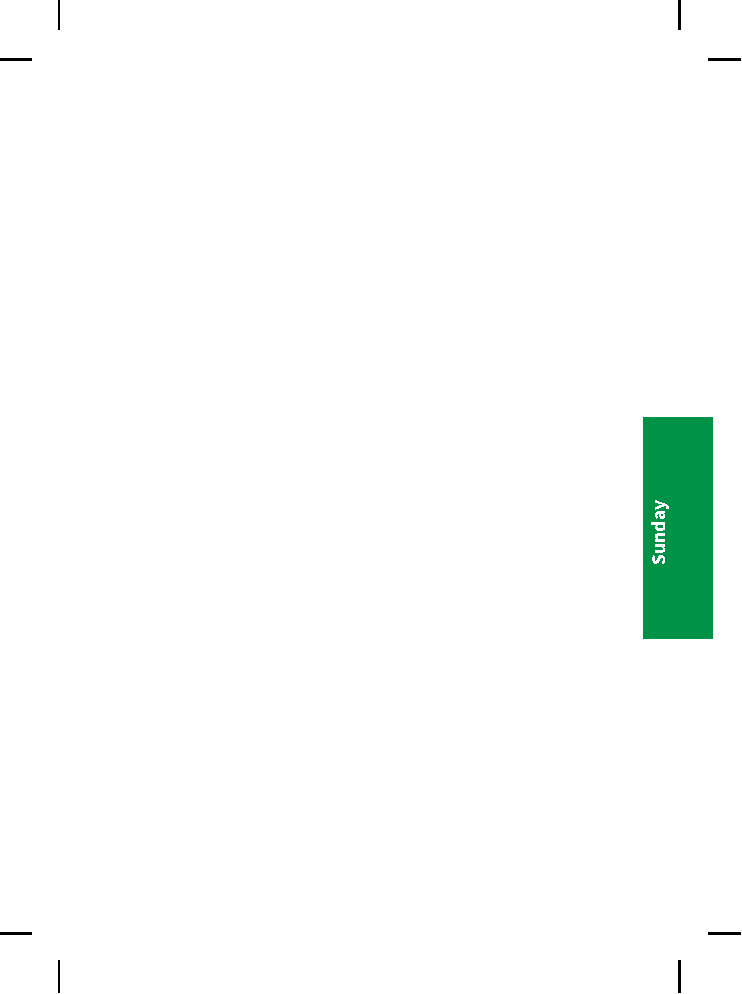
\includegraphics{wallpaper/sunday-odd-rotated.pdf}%
}]{sundayoddrotated}
\newpairofpagestyles[scrheadings]{sunday-table}{}
\AddLayersAtBeginOfPageStyle{sunday-table}{sundayeven}
\AddLayersAtBeginOfPageStyle{sunday-table}{sundayoddrotated}
\newpairofpagestyles[scrheadings]{sunday}{}
\AddLayersAtBeginOfPageStyle{sunday}{sundayeven}
\AddLayersAtBeginOfPageStyle{sunday}{sundayodd}

% define Monday page style
\DeclareNewLayer[background, oddpage,  width=125mm,%
height=169mm, contents={%
  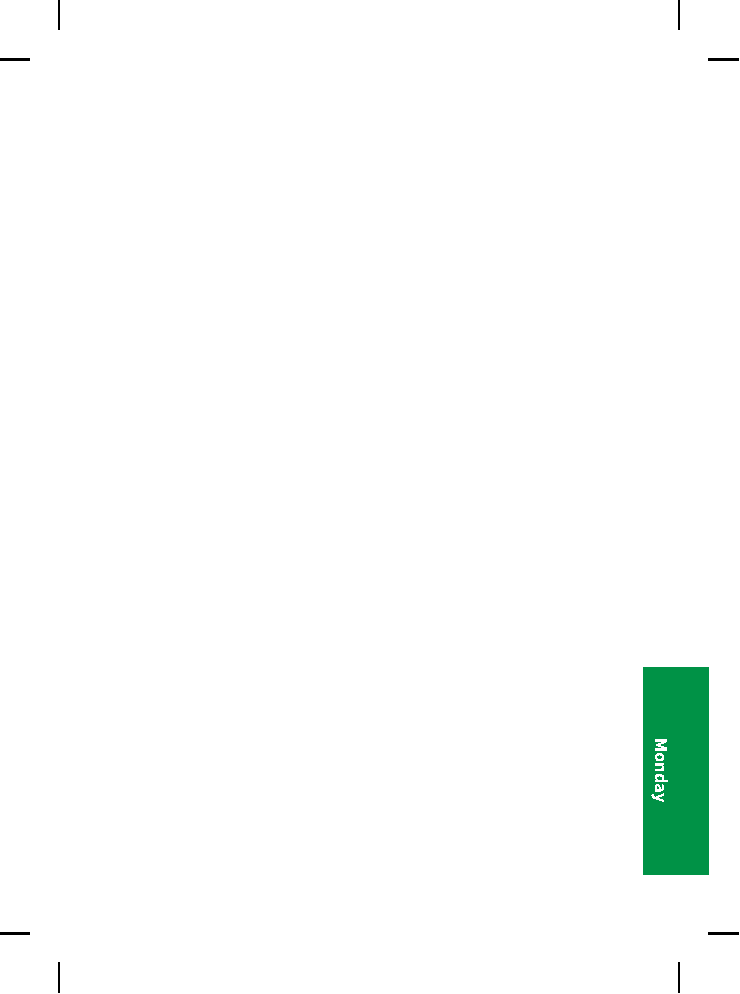
\includegraphics{wallpaper/monday-odd.pdf}%
}]{mondayodd}
\DeclareNewLayer[background, evenpage,  width=125mm,%
height=169mm, contents={%
  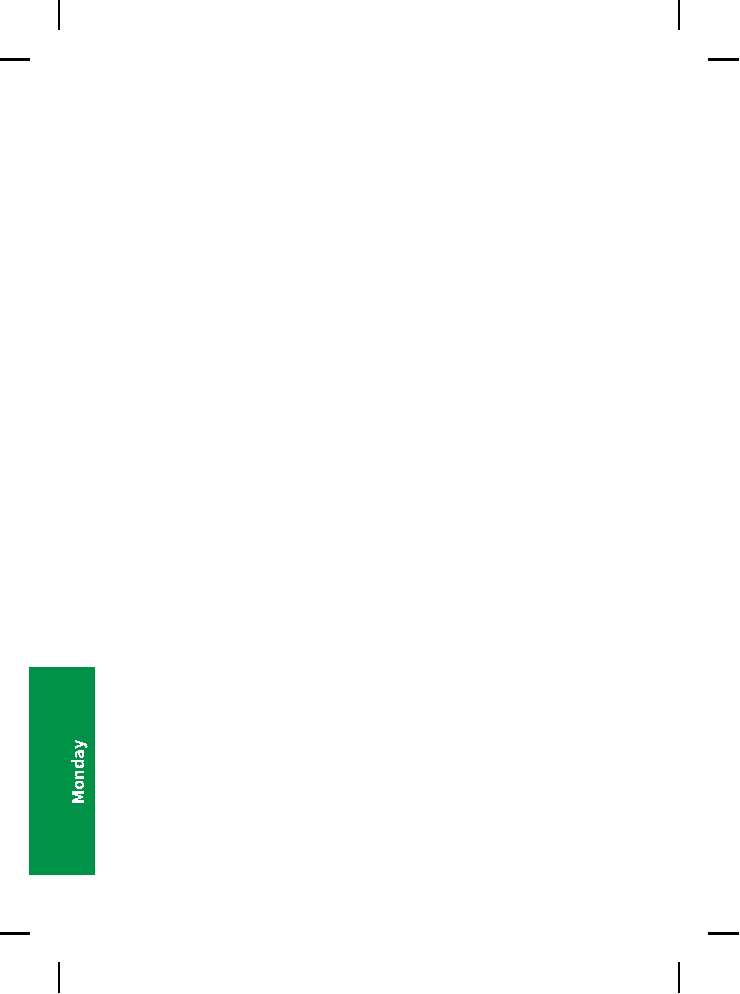
\includegraphics{wallpaper/monday-even.pdf}%
}]{mondayeven}
\DeclareNewLayer[background, oddpage,  width=125mm,%
height=169mm, contents={%
  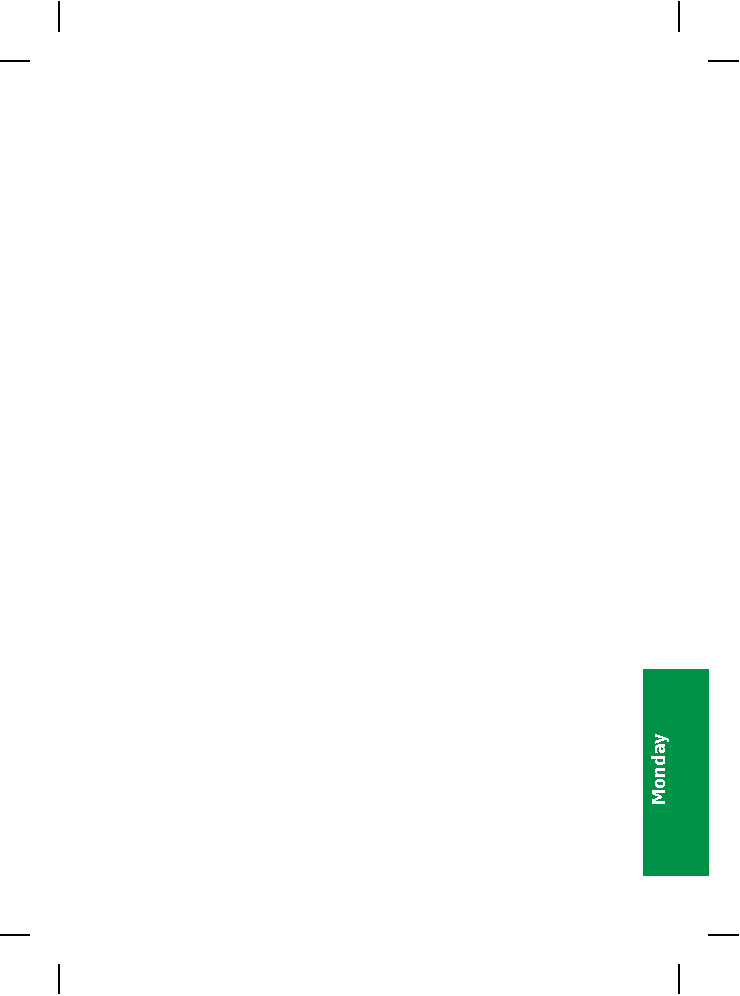
\includegraphics{wallpaper/monday-odd-rotated.pdf}%
}]{mondayoddrotated}
\newpairofpagestyles[scrheadings]{monday-table}{}
\AddLayersAtBeginOfPageStyle{monday-table}{mondayeven}
\AddLayersAtBeginOfPageStyle{monday-table}{mondayoddrotated}
\newpairofpagestyles[scrheadings]{monday}{}
\AddLayersAtBeginOfPageStyle{monday}{mondayeven}
\AddLayersAtBeginOfPageStyle{monday}{mondayodd}

% \setpagebackground selects the page style to be used depending on the current day. Each day has
% its own page style.
\newcommand{\setpagebackground}{ %
  \ifthenelse{\equal{\conferenceDay}{\saturday}}{%
    \pagestyle{saturday}
  }{}
  \ifthenelse{\equal{\conferenceDay}{\sunday}}{%
    \pagestyle{sunday}
  }{}
  \ifthenelse{\equal{\conferenceDay}{\monday}}{%
    \pagestyle{monday}
  }{}
}


% additional column type for tables
\newcolumntype{Y}[1]{>{\RaggedRight\arraybackslash}p{#1}}

%% length of the title boxes
\newlength{\titleboxwidth}
\setlength{\titleboxwidth}{\textwidth}
\advance\titleboxwidth by -6pt

% command to lay out the title boxes
\newcommand{\setabstract}[6]{
	% 1. speaker
	% 2. title
	% 3. subtitle
	% 4. abstract (Text)
	% 5. colour
	% 6. room
	%\thispagestyle{scrheadings}
  \setpagebackground
	\setlength\tabcolsep{0pt}
	% \setlength{\fboxsep}{0pt}
	\noindent\fcolorbox{white}{#5}{\parbox{\titleboxwidth}{%
		\noindent\begin{tabu}{X[5L]r}
			\isspeakerempty{#1}{#2}{#6}
			\issubtitleempty{#3}
		\end{tabu}%
	}}
	%
	\isabstractempty{#4}%
	\vspace{0.5em}% space to the next talk even if there is no abstract
	\setlength\tabcolsep{6pt} % set column padding back to default value
}

% lay out the speaker if there is any
% We assume that there is only a subtitle if the talk has a speaker.
\makeatletter
\newcommand{\isspeakerempty}[3]{%
	% Arguments:
	% 1. speaker
	% 2. title
	% 3. room
	\@ifmtarg{#1}{%
			\par\noindent\large \sectfont #2% % titel
			&
			#3, \talktime
			\tabularnewline
		}
		{
			\emph{#1} % Sprecher
			&
			\talktime
			\tabularnewline
			{\par\noindent\large \sectfont #2}% % titel
			&
			#3
			\tabularnewline
		}
		
}
\makeatother

% Lay out the subtitle
% has to be a separate function and has to be surrounded by \makeatletter for technical reasons
\makeatletter
\newcommand{\issubtitleempty}[1]{%
	\@ifnotmtarg{#1}{\multicolumn{2}{Y{\linewidth}}{\vspace{-0.6em} \noindent\bfseries \normalsize \sectfont #1}\tabularnewline}
}
\makeatother

% Lay out the abstract if there is any
% has to be a separate function and has to be surrounded by \makeatletter for technical reasons
\makeatletter
\newcommand{\isabstractempty}[1]{%
  \ifstrempty{#1}{%
    \vspace{1.5em}%
  }{%
    \vspace{0.5em}\newline%
    #1 \par% % abstract
    \vspace{1.5em}% space to the next talk even if there is an abstract
  }%
}
\makeatother

% define colours
\definecolor{deDonato}{cmyk}{0.16 0 .05 0}
\definecolor{two}{cmyk}{0.02 0 0.12 0.11}
\definecolor{academic}{cmyk}{0 0.02 0.23 0}
\definecolor{four}{cmyk}{0.35 0 0.33 0.16}
\definecolor{lightred}{cmyk}{0 .24 0.29 .04}

% session at De Donato
\newcommand{\abstractDeDonato}[4]%
{%
	\setabstract{#1}{#2}{#3}{#4}{deDonato}{De Donato}
}

% abstract at S.0.3
\newcommand{\abstractTwo}[4]%
{%
	\setabstract{#1}{#2}{#3}{#4}{two}{S.0.3}
}

% abstract at S.1.3
\newcommand{\abstractAcademic}[4]%
{%
	\setabstract{#1}{#2}{#3}{#4}{academic}{S.1.3}
}

% abstract at S.1.5
\newcommand{\abstractFour}[4]%
{%
	\setabstract{#1}{#2}{#3}{#4}{four}{S.1.5}
}

% abstract at a different location
\newcommand{\abstractOther}[5]%
{%
	\setabstract{#1}{#2}{#3}{#4}{commongray}{#5}
}

% box for workshops (they don't have an abstract in the booklet)
\newcommand{\workshopbox}[3]%
{%
	% 1. titel
	% 2. speaker
	% 3. Room
	\setlength\tabcolsep{0pt}
	\noindent\fcolorbox{white}{lightred}{\parbox{\titleboxwidth}{%
			\noindent
			\begin{tabu}{X[5L]r}
				\emph{#2} % speaker
				&
				\talktime
				\tabularnewline
				{\noindent\large \bfseries #1}% % title
				&
				#3
				\tabularnewline
			\end{tabu}
		}
	}
	\setlength\tabcolsep{6pt} % set column padding back to default
}

% too long
\newcommand{\tooLong}{Dieser Text ist viel zu lang. Dieser Text ist viel zu lang. Dieser Text ist viel zu lang. Dieser Text ist viel zu lang. Dieser Text ist viel zu lang. Dieser Text ist viel zu lang. Dieser Text ist viel zu lang. Dieser Text ist viel zu lang. Dieser Text ist viel zu lang. Dieser Text ist viel zu lang. Dieser Text ist viel zu lang. Dieser Text ist viel zu lang. Dieser Text ist viel zu lang. Dieser Text ist viel zu lang. }

\newlength{\fboxwidth}

\def\workshopsSection{workshopsSection}
\def\abstractsSection{abstractsSection}

% boxes for text-only advertisement texts by our sponsors
\newcommand{\sponsorenbox}[4]{%
  \setlength{\fboxwidth}{\textwidth}
  \advance\fboxwidth by -7.0pt
  \abstractSponsorenbox{#1}{#2}{#3}{#4}{\workshopsSection}%
}

\newcommand{\sponsorenboxA}[4]{%
  \setlength{\fboxwidth}{\textwidth}
  \advance\fboxwidth by -10.0pt
  \abstractSponsorenbox{#1}{#2}{#3}{#4}{\abstractsSection}%
}

%% box for advertisment by a sponsor
%% 1. logo
%% 2. width of the logo
%% 3. number of required lines of the logo (due to usage of wrapfigure)
%% 4. text
%% 5. Umfeld (\workshopsSection oder \abstractsSection}
\makeatletter
\newcommand{\abstractSponsorbox}[5]{%
  \setlength{\fboxsep}{4.5pt}%
  \noindent%
  \ifthenelse{\equal{#5}{\workshopsSection}}{%
    \hspace{2.65pt}%
  }{%
    \hspace{-1pt}%
  }%
  \fcolorbox{gray}{white}{%
    \parbox{\fboxwidth}{
    \@ifmtarg{#1}{}{%
      \begin{wrapfigure}[#3]{r}[0pt]{#2}
        \centering\vspace{-1\baselineskip}
        \includegraphics[width=#2]{#1}
      \end{wrapfigure}
    }

    \noindent #4
    }%
  }
  \setlength{\fboxsep}{3pt}
}
\makeatother

% definition of column types for the schedule tables
\newcolumntype{Z}[1]{>{\RaggedRight\arraybackslash}p{#1}}%
\newcolumntype{C}[1]{>{\Centering\arraybackslash}p{#1}}%

% common implementation of typesetting of a session in the tables
\newcommand{\talkInternal}[2]{%
  \textbf{#1}
  \ifthenelse{\equal{#2}{}}{}{%
    \newline\emph{#2}%
  }
}

% macro to typeset a talk in the schedule tables spanning over more than one row:
% usage: \longTalk{rowcount}{title}{speaker}
\newcommand{\longTalk}[3]{%
  &
  \multirow{#1}{\linewidth}{%
    \parbox{\linewidth}{
      %HACK Inserting a \vspace here is a dirty hack but it works.
      \vspace{0.45\baselineskip}
      \talkInternal{#2}{#3}%
    }
  }%
}%

% macro to typeset a talk in the schedule tables spanning over more than one row:
% usage: \talk{title}{speaker}
\newcommand{\talk}[2]{%
  &
  \talkInternal{#1}{#2}%
}%


\newcommand{\workshop}[3]%
{%
	\workshopbox{#1}{#2}{#3}
}%

\newcommand{\otherevent}[1]%
{%
	& \textbf{#1}
}%

\newcommand{\aulaevent}[2]%
{%
	&
	\multicolumn{3}{c}{
		\textbf{#1} (Aula) \par \emph{#2}
	}
}%

\newcommand{\coffeespace}{\vspace{0.4em}}
\newcommand{\workshopspace}{\vspace{0.5em}\\}

% define colors
\definecolor{commongray}{gray}{.9}
\renewcommand{\arraystretch}{1.4}



\begin{document}
\lsstyle
\usefont{T1}{DejaVuSansCondensed-TLF}{m}{n}
 
\pagestyle{cropmarksstyle}
\begin{titlepage}
  \thispagestyle{titlestyle}
  \null
\end{titlepage}
\pagestyle{cropmarksstyle}

\selectlanguage{english}
\section*{Content}

\vspace*{0.35em}%
\noindent Welcome\dotfill \pageref{welcome}

\vspace*{0.35em}%
\noindent Scholarships \dotfill \pageref{scholarships}

\vspace*{0.35em}%
\noindent Code of Conduct \dotfill \pageref{coc}

\vspace*{0.35em}%
\noindent Getting around in Milan\dotfill \pageref{getting-around}

\vspace*{0.35em}%
\noindent Saturday schedule\dotfill \pageref{saturday}

\vspace*{0.35em}%
\noindent Sunday schedule \dotfill \pageref{sunday}

\vspace*{0.35em}%
\noindent Monday schedule \dotfill \pageref{monday}

\vspace*{0.35em}%
\noindent Thank you \dotfill \pageref{thanks}

\vspace*{0.35em}%
\noindent Legal notice \dotfill \pageref{legal}

\vfill
\noindent
Hashtag: \#sotm

\vspace*{0.8em}%
\noindent
The general emergency telephone number in Italy is \textbf{112}.
\vfill

\newpage

\newpage
\section*{Welcome to Milan and to State of the Map 2018} \label{welcome}
This booklet gives you essential information
about the conference, the location and the schedule.  We are proud of the participation of the
OpenStreetMap community and our rich program but there is even more!  Please do get involved and
take advantage of the off-schedule sessions, discussions and spaces.

\paragraph*{The location} \label{welcome-location}
One room is available during the whole conference as free and open space offering chairs and tables
to talk to each other, work on your projects or just relax.  Two rooms are available for
self-organised sessions.  See page~\pageref{self-organised} for further information.  A floor plan
of the building can be found on page~\pageref{floorplan}.

\paragraph*{Help desk} \label{welcome-helpdesk}
You already know the registration desk, located at the ground floor (Building 3, same as the whole
conference).  It is also your port of call if you need support or help. We are listening to every
question, report and comment, related to the event, the code of conduct (page~\pageref{coc}) or any
aspect of the organisation.

\paragraph*{Sponsors} \label{welcome-sponsors}
We would like to thank our sponsors for making this event possible and for their support to the
OpenStreetMap Foundation.
\newpage

\newpage
\renewcommand{\arraystretch}{1.4}
\section*{Saturday Schedule}\label{saturday}
\renewcommand{\conferenceDay}{\saturday}
\setpagebackground
\begin{center}
  \noindent\begin{tabular}{Z{0.75cm}Z{6.85cm}}
    \cellcolor{commongray}
    &
    \multicolumn{1}{c}{
      \cellcolor{deDonato}
      De Donato
    }
    \tabularnewline
    \cellcolor{commongray}
    9:30
    \talk{Welcome}{}
    \tabularnewline
    \cellcolor{commongray}
    10:00
    \talk{Keynote OpenStreetMap—Now and into the Future}{Kate Chapman, Heather Leson}
    \tabularnewline
    \rowcolor{commongray}
  \end{tabular}

  \vspace{1.5\baselineskip}
  \noindent\begin{tabular}{Z{0.75cm}Z{3.0cm}Z{3.0cm}}
    \cellcolor{commongray}
    &
    \multicolumn{1}{c}{\cellcolor{deDonato} De Donato}
    & \multicolumn{1}{c}{\cellcolor{two} S.0.2}
    \tabularnewline
    \cellcolor{commongray}
    10:30
    \talk{Can we validate every change on OSM?}{Lukas Martinelli}
    \talk{Making Maps Without Databases}{Thomas Skowron}
    \tabularnewline
    \rowcolor{commongray}
    11:00 & \multicolumn{2}{c}{%
      \parbox[c]{24pt}{%
        
\includegraphics[height=10pt]{cafe}%
      }
      break} \tabularnewline
  \end{tabular}
\end{center}
  
\begin{center}
  \renewcommand{\arraystretch}{1.3}
  \noindent\begin{tabular}{Z{0.75cm}Z{2.0cm}Z{2.0cm}Z{2.0cm}}
    \cellcolor{commongray}
    & \multicolumn{1}{c}{\cellcolor{deDonato} De Donato}
    & \multicolumn{1}{c}{\cellcolor{two} S.0.3}
    & \multicolumn{1}{c}{\cellcolor{four} S.1.5}
    \tabularnewline
    \cellcolor{commongray}
    11:30
    \talk{Interpreting Imagery for OpenStreetMap}{Chad Blevins}
    \talk{OpenMapTiles: Vector tiles from OpenStreetMap}{Petr Pridal, Jiri Komarek}
    \talk{Qt to create Maps}{Paolo Angelelli}
    \tabularnewline
  \end{tabular}
\end{center}
  
\begin{center}
  \renewcommand{\arraystretch}{1.3}
  \noindent\begin{tabular}{Z{0.75cm}Z{2.0cm}Z{2.0cm}Z{2.0cm}}
    \cellcolor{commongray}
    & \multicolumn{1}{c}{\cellcolor{deDonato} De Donato}
    & \multicolumn{1}{c}{\cellcolor{two} S.0.3}
    & \multicolumn{1}{c}{\cellcolor{four} S.1.5}
    \tabularnewline
    \cellcolor{commongray}
    12:00
    %\talk{Advertising mapping: using OpenStreepMap for the protection of landscape}{Paul Desgranges}
    \talk{Advertising mapping}{Paul Desgranges}
    \talk{Large Scale Deep Learning for Map Making}{Alina Negreanu and Bogdan Gliga}
    \talk{Field Mapping tools and technologies}{Paul Uithol}
    \tabularnewline
    \cellcolor{commongray}
    12:30
    \talk{An excursion in to the world of OSM tagging presets}{Simon Poole}
    \talk{How Deep Learning could help to improve OSM Data Quality?}{Oliver Courtin}
    \tabularnewline
    \rowcolor{commongray}
    13:00 & \multicolumn{3}{c}{%
    \parbox[c]{24pt}{%
      
\includegraphics[height=10pt]{restaurant}%
    }
    lunch} \tabularnewline
    \rowcolor{commongray}
    14:00
    & \multicolumn{3}{c}{photo}
    \tabularnewline
    \cellcolor{commongray}
    14:10
    \talk{Addressing addresses}{Sarah Hoffmann}
    % \talk{The Belgian perspective to building OpenStreetMap community}{Ben Abelshausen, Joost Schouppe}
    \talk{Belgian perspective to building OSM community}{Ben Abels\-hausen, Joost Schouppe}
    \talk{Lightning Talks 1}{}
    \tabularnewline
  \end{tabular}
\end{center}
  
\begin{center}
  \renewcommand{\arraystretch}{1.3}
  \noindent\begin{tabular}{Z{0.75cm}Z{2.0cm}Z{2.0cm}Z{2.0cm}}
    \cellcolor{commongray}
    & \multicolumn{1}{c}{\cellcolor{deDonato} De Donato}
    & \multicolumn{1}{c}{\cellcolor{two} S.0.3}
    & \multicolumn{1}{c}{\cellcolor{four} S.1.5}
    \tabularnewline
    \cellcolor{commongray}
    14:40
    \talk{2, 4, 6, 8, Here's how we interpolate}{Julian Simioni}
    % \talk{A new approach to garner prolific contribution in OpenStreetMap}{Kshitiz Khanal}
    \talk{New approach to garner prolific contribution in OSM}{Kshitiz Khanal}
    \talk{The LWG Presents: GDPR Implementation for OSM}{Kathleen Lu}
    \tabularnewline
    \cellcolor{commongray}
    15:10
    \talk{OsmAnd making live maps update}{Victor Shcerb}
    \talk{Building up the Microsoft Open Maps Team}{Osin Herriott}
    \tabularnewline
    \rowcolor{commongray}
    15:40
    & \multicolumn{3}{c}{%
    \parbox[c]{24pt}{%
      
\includegraphics[height=10pt]{cafe}%
    }
    break} \tabularnewline
    \cellcolor{commongray}
    16:10
    \talk{Lies, damned lies, and OSM statistics}{Frederik Ramm}
    \talk{Verifying Our Edits}{Bogdan Petrea, Armin Gheorghina}
    \talk{Corporate Cartography: How the sausage gets made}{Paul Norman}
    \tabularnewline
  \end{tabular}
\end{center}
  
\begin{center}
  \renewcommand{\arraystretch}{1.3}
  \noindent\begin{tabular}{Z{0.75cm}Z{2.0cm}Z{2.0cm}Z{2.0cm}}
    \cellcolor{commongray}
    & \multicolumn{1}{c}{\cellcolor{deDonato} De Donato}
    & \multicolumn{1}{c}{\cellcolor{two} S.0.3}
    & \multicolumn{1}{c}{\cellcolor{four} S.1.5}
    \tabularnewline
    \cellcolor{commongray}
    16:40
    \talk{An innovative approach to support OSM data generation}{Emanuela Mihut}
    \talk{Mapping Competition with Focus on Quality: Lesson Learned}{Yantisa Akhadi}
    \talk{Open Gender Monologues}{Heather Leson}
    \tabularnewline
    \cellcolor{commongray}
    17:10
    \talk{Pinpointing the power grid}{Sajjad Anwar}
    \talk{Improving OSMCha for the community}{Wille Marcel Lima Malheiro}
    \tabularnewline
    \rowcolor{commongray}
    19:30
    &
    \multicolumn{3}{c}{%
      \parbox[c]{24pt}{%
        
\includegraphics[height=10pt]{restaurant}%
      }%
      Social Event at Old Fashion Milano%
    }
    \tabularnewline
  \end{tabular}
\end{center}
\renewcommand{\arraystretch}{1.0}

\newpage
\renewcommand{\arraystretch}{1.4}
\renewcommand{\conferenceDay}{\sunday}
\setpagebackground
\pagestyle{sunday-table}
\newgeometry{
  paperwidth=125mm,
  paperheight=168mm, 
  portrait,
  top=22mm,
  inner=20mm, % usually 22mm
  outer=17mm, % usually 20mm
  bottom=25mm,
  headsep=3mm,
  footskip=12mm
}
\noindent\begin{landscape}
  %\section*{Sessions on Sunday}
  \label{sunday}
  \noindent\begin{center}
    \noindent\begin{tabular}{Z{0.75cm}Z{2.2cm}Z{2.4cm}Z{2.8cm}Z{2.2cm}}
    %\noindent\begin{tabular}{Z{0.75cm}Z{2.0cm}Z{2.0cm}Z{2.8cm}Z{2.0cm}}
      \cellcolor{commongray}
      & \multicolumn{1}{c}{\cellcolor{deDonato} De Donato}
      & \multicolumn{1}{c}{\cellcolor{two} S.0.3}
      & \multicolumn{1}{c}{\cellcolor{academic} S.1.3}
      & \multicolumn{1}{c}{\cellcolor{four} S.1.3}
      \tabularnewline
      \cellcolor{commongray}
      09:30
      \talk{Alternative perspectives through artistic interpretations}{Sebastian Meier et.\,al.}
      \talk{What's up with the public transport}{Ilya Zverev}
      %\talk{Coordinating improved communication between the academic and OpenStreetMap communities}{Peter Mooney et.\,al.}
      \talk{Communication between academic and OSM communities}{Peter Mooney et.\,al.}
      \tabularnewline
      \cellcolor{commongray}
      10:00
      \talk{Lightning Talks 2}{}
      \talk{Network for transport open data}{Céline Jacquin}
      %\talk{Surveying OSM contributors: Learning from the community}{Zoe Gardner et.\,al.}
      \talk{Surveying OSM contributors}{Zoe Gardner et.\,al.}
      \talk{Thematic mapping with emojis}{Erik Escoffier}
      \tabularnewline
      \cellcolor{commongray}
      10:30
      \talk{Lightning Talks 3}{}
      \talk{Solving routing problems with OSM and VROOM}{}
      %\talk{Solving vehicle routing problems with OpenStreetMap and VROOM}{}
      \talk{Slum health mapping as catalyst~\dots}{João Porto de Albuquerque et.\,al.}
      %\talk{Slum health mapping as catalyst for a collaborative agenda for research, practice, local citizens and volunteers}{João Porto de Albuquerque et.\,al.}
      \talk{Open\-Street\-Map My Business}{Stefan Keller}
      \tabularnewline
    \end{tabular}
  \end{center}
  \begin{center}
    \noindent\begin{tabular}{Z{0.75cm}Z{2.2cm}Z{2.4cm}Z{2.8cm}Z{2.2cm}}
    %\noindent\begin{tabular}{Z{0.75cm}Z{2.0cm}Z{2.0cm}Z{2.8cm}Z{2.0cm}}
      \cellcolor{commongray}
      & \multicolumn{1}{c}{\cellcolor{deDonato} De Donato}
      & \multicolumn{1}{c}{\cellcolor{two} S.0.3}
      & \multicolumn{1}{c}{\cellcolor{academic} S.1.3}
      & \multicolumn{1}{c}{\cellcolor{four} S.1.3}
      \tabularnewline
      \rowcolor{commongray}
      11:00
      & \multicolumn{4}{c}{%
      \parbox[c]{24pt}{%
        
\includegraphics[height=10pt]{cafe}%
      }
      break}
      \tabularnewline
      \cellcolor{commongray}
      11:30
      \talk{OSM and the European agenda}{Vlado Cetl}
      %\talk{The use of OSM in public transport in Helsinki, Finland}{Markku Huotari}
      \talk{The use of OSM in public transport in Helsinki}{Markku Huotari}
      %\talk{Human-Centered Data Science and OpenStreetMap: Contributor-Centric OpenStreetMap Analysis Infrastructure}{Jennings Anderson}
      \talk{Contributor-Centric OSM Analysis Infrastructure}{Jennings Anderson}
      \talk{Some Location Intelligence from OSM}{Jaak Laineste}
      \tabularnewline
      \cellcolor{commongray}
      12:00
      \longTalk{2}{Sustainability of OSM Mapping Projects}{Robert Soden}
      \talk{Printing OSM Maps}{Hartmut Holzgraefe}
      %\talk{Intrinsic assessment of the temporal accuracy, up-to-dateness, lineage and thematic accuracy of OpenStreetMap}{Francesco Frassinelli}
      \talk{Intrinsic assessment of the accuracy of OSM}{Francesco Frassinelli et.\,al.}
      \longTalk{2}{Humans and Machines Mapping Together}{Zhuangfang NaNa Yi}
      \tabularnewline
      \cellcolor{commongray}
      12:30
      &
      \talk{Osmose-QA and validation with JOSM}{Fr\'{e}d\'{e}ric Rodrigo}
      %\talk{Osmose-QA \& Common validation with JOSM}{Fr\'{e}d\'{e}ric Rodrigo}
      \talk{Comprehensive OSM History Analyses}{Michael Auer et.\,al.}
      %\talk{Comprehensive OpenStreetMap History Data Analyses- for and with the OSM community}{Michael Auer et.\,al.}
      &
    \end{tabular}
  \end{center}
  \begin{center}
    \noindent\begin{tabular}{Z{0.75cm}Z{2.2cm}Z{2.4cm}Z{2.8cm}Z{2.2cm}}
    %\noindent\begin{tabular}{Z{0.75cm}Z{2.0cm}Z{2.0cm}Z{2.8cm}Z{2.0cm}}
      \cellcolor{commongray}
      & \multicolumn{1}{c}{\cellcolor{deDonato} De Donato}
      & \multicolumn{1}{c}{\cellcolor{two} S.0.3}
      & \multicolumn{1}{c}{\cellcolor{academic} S.1.3}
      & \multicolumn{1}{c}{\cellcolor{four} S.1.3}
      \tabularnewline
      \rowcolor{commongray}
      13:00
      & \multicolumn{4}{c}{%
        \parbox[c]{24pt}{%
          
\includegraphics[height=10pt]{restaurant}%
        }
      lunch}
      \tabularnewline
      \cellcolor{commongray}
      14:00
      \longTalk{2}{The road towards diversity in OSM still needs to be mapped}{Selene Yang}
      \talk{Navigating  with OSM in Bangladesh}{Tasauf A Baki Billah}
      %\talk{Pathao: Navigating  with OSM in Bangladesh while Community blends in with Corporate}{Tasauf A Baki Billah}
      \talk{Innovative approach to support OSM mapping}{Emanuela Mihut et.\,al.}
      %\talk{An innovative approach to support OSM data generation}{Emanuela Mihut et.\,al.}
      \longTalk{2}{Exploring OSM's history using the ohsome data analytics platform}{Martin Raifer et.\,al.}
      \tabularnewline
      \cellcolor{commongray}
      14:30
      &
      \talk{Flying ferries and moving pavements?}{Guillaume Rischard}
      %\talk{Flying ferries and moving pavements? Pedestrian routing on rare modes of transport}{Guillaume Rischard}
      \talk{Osm\-Event\-Analyst}{Luca Delucchi et.\,al.}
      %\talk{Investigating the OSM mapping process after disasters: OsmEventAnalyst and its application for the 2016 Italian earthquakes}{Luca Delucchi et.\,al.}
      &
      \tabularnewline
      \cellcolor{commongray}
      15:00
      \talk{Lightning Talks 4}{}
      \talk{CityZen}{Redon Skikuli}
      %\talk{Privacy aware city navigation with CityZen app}{Redon Skikuli}
      \talk{Areas-of-Interest for OSM}{Stefan Keller}
      %\talk{Areas-of-Interest for OpenStreetMap with Big Spatial Data Analytics}{Stefan Keller}
      \talk{IT backend of the OSM community}{Timofey}
      %\talk{IT backend of the OpenStreetMap community}{Timofey}
      \tabularnewline
    \end{tabular}
  \end{center}
  \begin{center}
    \noindent\begin{tabular}{Z{0.75cm}Z{2.2cm}Z{2.4cm}Z{2.8cm}Z{2.2cm}}
    %\noindent\begin{tabular}{Z{0.75cm}Z{2.0cm}Z{2.0cm}Z{2.8cm}Z{2.0cm}}
      \cellcolor{commongray}
      & \multicolumn{1}{c}{\cellcolor{deDonato} De Donato}
      & \multicolumn{1}{c}{\cellcolor{two} S.0.3}
      & \multicolumn{1}{c}{\cellcolor{academic} S.1.3}
      & \multicolumn{1}{c}{\cellcolor{four} S.1.3}
      \tabularnewline
      \rowcolor{commongray}
      15:30
      & \multicolumn{4}{c}{%
      \parbox[c]{24pt}{%
        
\includegraphics[height=10pt]{cafe}%
      }
      break}
      \tabularnewline
      \cellcolor{commongray}
      16:00
      \talk{A tale of two (mapping) cities}{Alsino Skow\-ron\-nek et.\,al.}
      %\talk{A tale of two (mapping) cities}{Alsino Skow\-ron\-nek, Mi\-chele Ferretti}
      \talk{Lightning Talks 5}{}
      \talk{Using OSM for land\-use/landc\-over maps}{Cidália C. Fonte}
      %\talk{Potential and limitation of using OSM data for the creation/validation of Land Use/Cover maps}{Cidália C. Fonte}
      \talk{}{}
      \tabularnewline
      \cellcolor{commongray}
      16:30
      \talk{OSM Community Grants: sharing experiences}{Rebecca Firth}
      \talk{Lightning Talks 6}{}
      \talk{A resource mapping framework based upon OSM}{Chris Emberson et.\,al.}
      %\talk{The challenges and issues associated with a natural resource mapping framework based upon OpenStreetMap}{Chris Emberson et.\,al.}
      \longTalk{2}{Navigation Mapping Workshop}{Kajari Ghosh}
      \tabularnewline
      \cellcolor{commongray}
      17:00
      \talk{Working with the Comunity}{Ryan Peterson}
      \talk{Lightning Talks 7}{}
      \talk{Modeling bicycle traffic}{Dominik Ziemke et.\,al.}
      %\talk{Using OpenStreetMap to model bicycle traffic in an agent-based transport simulation}{Dominik Ziemke et.\,al.}
      &
      \tabularnewline
    \end{tabular}
  \end{center}
\end{landscape}
\renewcommand{\arraystretch}{1.0}
\justifying
\restoregeometry
\setpagebackground

\newpage
\renewcommand{\arraystretch}{1.4}
\renewcommand{\conferenceDay}{\sunday}
\setpagebackground
\pagestyle{monday-table}
\newgeometry{
  paperwidth=125mm,
  paperheight=168mm, 
  portrait,
  top=22mm,
  inner=20mm, % usually 22mm
  outer=17mm, % usually 20mm
  bottom=25mm,
  headsep=3mm,
  footskip=12mm
}
\noindent\begin{landscape}
  %\section*{Sessions on Monday}
  \label{monday}
  \noindent\begin{center}
    \noindent\begin{tabular}{Z{0.75cm}Z{2.9cm}Z{2.9cm}Z{2.9cm}}
      \cellcolor{commongray}
      & \multicolumn{1}{c}{\cellcolor{deDonato} De Donato}
      & \multicolumn{1}{c}{\cellcolor{two} S.0.3}
      & \multicolumn{1}{c}{\cellcolor{four} S.1.3}
      \tabularnewline
      \cellcolor{commongray}
      09:30
      \talk{Completing the Map with Street-level Imagery}{Christopher Beddow}
      \talk{Road Completion in Belgium}{Ben Abelshausen}
      %\talk{Road Completion in Belgium - Mapping \& verifying all the roads}{Ben Abelshausen}
      \talk{Lightning Talks 8}{}
      \tabularnewline
      \cellcolor{commongray}
      10:00
      \talk{Pic4Review: fun OSM editing based on street pictures}{Adrien Pavie}
      \talk{Going to Production with OpenStreeetMap at Microsoft}{Jubal Harpster}
      \longTalk{3}{Building your OSM web app in minutes with vector tiles}{Lukas Martinelli, Jinal Foflia}
      \tabularnewline
      \cellcolor{commongray}
      10:30
      \talk{Form \& Map based Mobile Tool for Survey and Validation}{Kuo-Yu slayer Chuang}
      %\talk{Form \& Map based Mobile OSM Tool for Field Survey and Validation}{Kuo-Yu slayer Chuang}
      \talk{Switch2OSM: A real enterprise context case study}{Andrea Capata}
      &
      \tabularnewline
    \end{tabular}
  \end{center}
  \noindent\begin{center}
    \noindent\begin{tabular}{Z{0.75cm}Z{2.9cm}Z{2.9cm}Z{2.9cm}}
      \cellcolor{commongray}
      & \multicolumn{1}{c}{\cellcolor{deDonato} De Donato}
      & \multicolumn{1}{c}{\cellcolor{two} S.0.3}
      & \multicolumn{1}{c}{\cellcolor{four} S.1.3}
      \tabularnewline
      \rowcolor{commongray}
      11:00
      & \multicolumn{3}{c}{%
        \parbox[c]{24pt}{%
          
\includegraphics[height=10pt]{cafe}%
        }
      break}
      \tabularnewline
      \cellcolor{commongray}
      11:30
      \talk{The new Wheelmap}{Svenja Heinecke}
      %\talk{The new Wheelmap: Joining forces in accessibility mapping – feat.: "I Wheel Share"}{Svenja Heinecke}
      \talk{Making bot edits safe and acceptable}{Yuri Astrakhan}
      \longTalk{2}{OpenStreetMap and the future of transport}{Michele Ferretti}
      \tabularnewline
      \cellcolor{commongray}
      12:00
      \talk{Modding the OSM Data Model}{Jochen Topf}
      \talk{Robot Tracers}{Nikola Trifunovic}
      %\talk{Robot Tracers - Extraction and Classification at scale using \& CNTK}{Nikola Trifunovic}
      &
      \tabularnewline
      \cellcolor{commongray}
      12:30
      \talk{Energy efficient routing with OSM}{Arndt Brenschede}
      \talk{Reaching out to vulnerable communities in Turkey}{Gülşah Eker}
      \talk{Attracting students with Google Summer of Code}{Peter Barth}
      \tabularnewline
      \rowcolor{commongray}
      13:00
      & \multicolumn{3}{c}{%
        \parbox[c]{24pt}{%
          
\includegraphics[height=10pt]{restaurant}%
        }
      lunch}
      \tabularnewline
    \end{tabular}
  \end{center}
\end{landscape}
\renewcommand{\arraystretch}{1.0}
\justifying
\restoregeometry
\setpagebackground

\newpage
\pagestyle{metro}
\null
\label{metromap}

\newpage
\section*{Legal Notice}
\label{legal}
\pagestyle{cropmarksstyle}

\RaggedRight
{\small
  State of the Map 2018 is jointly organised by the OpenStreetMap Foundation,
  Politecnico di Milano and Wikimedia Italia.

\vspace{0.5em}
\newlength\logoHeight
\setlength{\logoHeight}{3.5\baselineskip}

\includegraphics[height=\logoHeight]{osm-logo.pdf}
\hspace{1em}

\includegraphics[height=\logoHeight]{wikimedia_italia.pdf}

\vspace{0.5em}
\noindent Responsible for the content:\\
OpenStreetMap Foundation\\
132 Maney Hill Road\\
Sutton Coldfield\\
West Midlands B72 1JU\\
United Kingdom

\vspace{0.5em}
\noindent This booklet has been prepared using Lua\LaTeX\ and 
other free and open source software.\\
Source code: github.com/osmfoundation/sotm2018-booklet\\
\noindent Typesetting and layout: Michael Reichert\\
Map data: 
\includegraphics[height=7pt]{copyright}~Open\-Street\-Map contributors, osm.org/copyright\\
Icons in the schedule: SJJB Management, CC-0\\
Copyeditors: TBA\\

\vspace{1em}
\noindent \begin{minipage}[htbp]{0.2\textwidth}
\noindent
\includegraphics[width=\linewidth]{cc-by-sa-pdf}
\end{minipage}
\hfill
\begin{minipage}[hbtp]{0.74\textwidth}\RaggedRight
  {\small
    This booklet may be re-used under the Creative Commons Attribution Share-Alike 3.0 license.
    This does not apply to advertisements and logos of companies and organisations.
  }
\end{minipage}

%\includepdf{wallpaper/rueckseite.pdf}


\end{document}
